\section{Vector spaces}

We're used to thinking of vectors as something like
%
\[\begin{bmatrix}
    3 \\ 5
\end{bmatrix}\]
%
or
%
\begin{figure}[H]
    \centering

    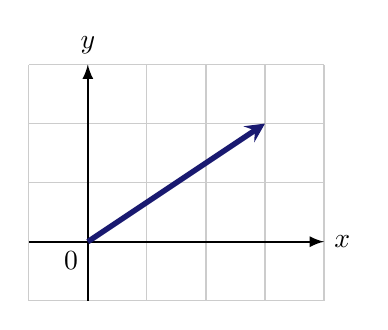
\begin{tikzpicture}[scale=0.75]
        \draw[thin,gray!40] (-1,-1) grid (4, 3);
        \draw[thick, ->, >=latex] (-1,0)--(4,0) node[right]{\(x\)};
        \draw[thick, ->, >=latex] (0,-1)--(0,3) node[above]{\(y\)};
        \draw (0, 0) node[below left] {0};
        
        \draw[line width=2pt, MidnightBlue, -stealth] (0,0)--(3,2);        
    \end{tikzpicture}
\end{figure}
%
but this is only a fraction of what the term ``vector'' encompasses. As we shall see in this section, given the correct prerequisites, even something like
%
\[
    2x^2 + 3x + 5
\]
%
can be a vector!



\subsection{What is a vector space?}

To start, we define a \textit{vector space} as follows.
%
\begin{quote}
    \textbf{Definition of a vector space.}

    For a field \(K\), a non-empty set \(V\) is a \(K\)-vector space (or a vector space over \(K\)) if, for any \(\vec{u}, \vec{v} \in V\) and any scalar \(a \in K\), we have
    %
    \begin{align*}
        \vec{u} + \vec{v} &\in V \tag{closure under vector addition}\\
        a\vec{u} &\in V \tag{closure under scalar multiplication}
    \end{align*}
    %
    The elements of \(V\) are called \textit{vectors}.
\end{quote}

We note the following:
%
\begin{itemize}
    \item Here, \(K\) is a \textit{field}, typically either \(\mathbb{R}\) or \(\mathbb{C}\). This field tells us what counts as a ``scalar'' in this vector space.
    \item The pair of properties listed in the definition give rise to what's called \textit{linearity} --- it's what makes linear algebra linear.
    \item Vector addition and scalar multiplication are governed by the following rules.
    %
    \begin{align*}
        (a + b)\vec{v} &= a\vec{v} + b\vec{v}\\
        (a(b \vec{v})) &= (ab) \vec{v}\\
        \vec{u} + \vec{v} &= \vec{v} + \vec{u}\\
        \vec{u} + (\vec{v} + \vec{w}) &= (\vec{u} + \vec{v}) + \vec{w}\\
        a(\vec{u} + \vec{v}) &= a\vec{u} + a\vec{v}\\
        \vec{v} &= \vec{v} + \vec{0}\\
        0\vec{v} &= \vec{0}\\
        1\vec{v} &= \vec{v}
    \end{align*}
    %
    where \(\vec{u}, \vec{v}, \vec{w}\) are vectors, \(a, b\) are scalars in \(K\), and \(\vec{0}\) represents the zero vector.
\end{itemize}





\subsection{Examples of vector spaces}

Based on the definition above, what counts as a vector space? (For now, let us set \(K = \mathbb{R}\) and consider only \(\mathbb{R}\)-vector spaces.)

Unsurprisingly, the set of pairs of real numbers, denoted as \(\mathbb{R}^2\), is a vector space:
%
\[
    \mathbb{R}^2 =
    \left\{
    \left.
    \begin{bmatrix}
        x \\ y
    \end{bmatrix}
    \right|
    x, y \in \mathbb{R}
    \right\}
\]
%
and each of the pairs \(\begin{bmatrix} x \\ y \end{bmatrix}\) is a vector. This is because of the fact that the sum of any two vectors in \(\mathbb{R}^2\) must also be in \(\mathbb{R}^2\), and that the scaled version of any vector in \(\mathbb{R}^2\) must also be in \(\mathbb{R}^2\). These vectors can be visualised as arrows in 2D space, as shown in figures \ref{fig:Ch03-r2-vectors-closed-under-addition} and \ref{fig:Ch03-r2-vectors-closed-under-scaling}.

\begin{figure}[H]
    \centering

    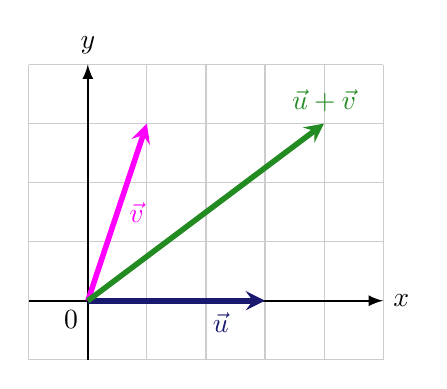
\begin{tikzpicture}[scale=0.75]
        \draw[thin,gray!40] (-1,-1) grid (5, 4);
        \draw[thick, ->, >=latex] (-1,0)--(5,0) node[right]{\(x\)};
        \draw[thick, ->, >=latex] (0,-1)--(0,4) node[above]{\(y\)};
        \draw (0, 0) node[below left] {0};
        
        \draw[line width=2pt, MidnightBlue, -stealth] (0,0)--(3,0) node[pos=3/4, below]{\(\vec{u}\)};
        
        \draw[line width=2pt, Fuchsia, -stealth] (0,0)--(1,3) node[pos=1/2, anchor=west]{\(\vec{v}\)};    
        
        \draw[line width=2pt, ForestGreen, -stealth] (0,0)--(4,3) node[above]{\(\vec{u}+\vec{v}\)};
    \end{tikzpicture}
    
    \caption{Vectors in \(\mathbb{R}^2\) are closed under addition. For any given pair of vectors \(\vec{u}\) and \(\vec{v}\) both in \(V\), their sum \(\vec{u} + \vec{v}\) must also be a vector.}
    \label{fig:Ch03-r2-vectors-closed-under-addition}
\end{figure}

\begin{figure}[H]
    \centering

    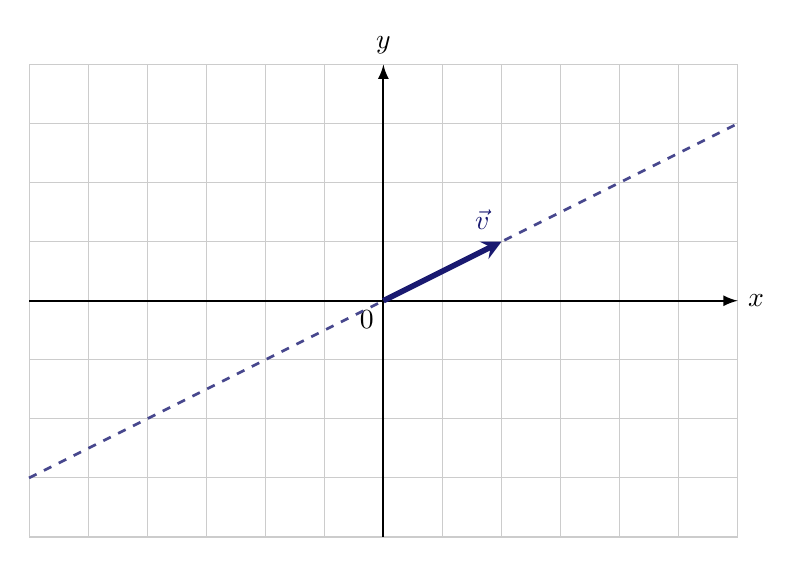
\begin{tikzpicture}[scale=0.75]
        \draw[thin,gray!40] (-6,-4) grid (6, 4);
        \draw[thick, ->, >=latex] (-6,0)--(6,0) node[right]{\(x\)};
        \draw[thick, ->, >=latex] (0,-4)--(0,4) node[above]{\(y\)};
        \draw (0, 0) node[below left] {0};

        \draw[dashed, line width=1pt, MidnightBlue!80] (-6,-3)--(6,3); 
        \draw[line width=2pt, MidnightBlue, -stealth] (0,0)--(2,1) node[above left] {\(\vec{v}\)};
         
    \end{tikzpicture}
    
    \caption{Vectors in \(\mathbb{R}^2\) are closed under scalar multiplication. For any given vector \(v \in \mathbb{R}^2\), the product between \(\vec{v}\) and any scalar \(a\) (i.e. any vector lying on the dashed line) is also a vector.}
    \label{fig:Ch03-r2-vectors-closed-under-scaling}
\end{figure}





The same goes with the set of triplets of real numbers
%
\(
\begin{bmatrix}
    x \\ y \\ z
\end{bmatrix}\),
%
which is denoted as \(\mathbb{R}^3\) and whose vectors can be visualised as arrows in 3D space. In fact, for any natural number \(n\), the set of \(n\)-tuples of real numbers (denoted as \(\mathbb{R}^n\)) is a vector space.

So far this is not very exciting as it is equivalent to our usual notion of what a ``vector'' is. To step things up a notch, let us  consider the set of polynomials of degree at most \(2\). Is this set a vector space?
%
\[
    \{ax^2 + bx + c \mid a, b, c, \in \mathbb{R}\}
\]
%
To answer this, we notice that:
%
\begin{itemize}
    \item Given any two polynomials in this set,
    %
    \begin{align*}
        \alpha &= a_1 x^2 + b_1 x + c_1\\
        \beta &= a_2 x^2 + b_2 x + c_2
    \end{align*}
    %
    their sum \(\alpha + \beta\) must also be an element of this set.

    \item If we multiply a polynomial of degree at most 2 with a scalar \(a\), the resultant product must also be a polynomial of degree at most 2.
\end{itemize}
%
This means that this set is indeed a vector space!

Table \ref{tab:Ch03-vector-space-examples} lists some examples of sets that are vector spaces, and some that aren't.

\begin{table}[H]
    \centering
    \begin{tabular}{|c|c|}
        \hline
        \textbf{Vector spaces} & \textbf{Not vector spaces}\\
        \hline
        The set of real numbers \(\mathbb{R}\) & The set of natural numbers \(\mathbb{N}\)\\
        The set of complex numbers \(\mathbb{C}\) & The set of polynomials of degree exactly 2\\
        The set of continuous functions that act on \(\mathbb{R}\) & The set of irrational numbers \(\mathbb{R} \setminus \mathbb{Q}\)\\
        \hline
    \end{tabular}
    \caption{Some sets are vector spaces while some are not.}
    \label{tab:Ch03-vector-space-examples}
\end{table}


Our previous definition of a vector space consisted of two properties. We can group those properties together to produce the following alternative but equivalent definition.
%
\begin{quote}
    \textbf{Alternative definition of a vector space.}

    For a field \(K\) (typically \(\mathbb{R}\) or \(\mathbb{C}\)), a non-empty set \(V\) is a \(K\)-vector space if, for any \(\vec{u}, \vec{v} \in V\) and any scalar \(a \in K\), we have \(a\vec{u} + \vec{v} \in V\).
\end{quote}

A vector space always contains a zero vector. This can be shown by setting \(\vec{u} = \vec{v}\) and \(a = -1\) in the definition above.




\subsection{Collinearity, span and subspaces}

Vectors \(\vec{u}\) and \(\vec{v}\) are said to be collinear if \(\vec{u} = a\vec{v}\) for some scalar \(a\). See figure \ref{fig:Ch03-collinearity}.

\begin{figure}[H]
    \centering

    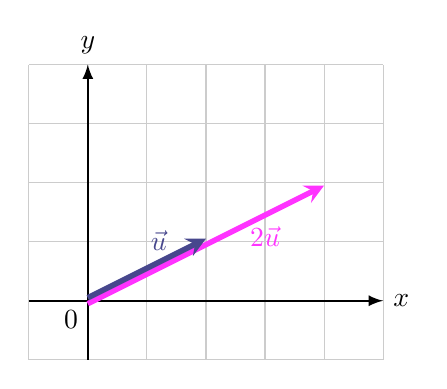
\begin{tikzpicture}[scale=0.75]
        \draw[thin,gray!40] (-1,-1) grid (5, 4);
        \draw[thick, ->, >=latex] (-1,0)--(5,0) node[right]{\(x\)};
        \draw[thick, ->, >=latex] (0,-1)--(0,4) node[above]{\(y\)};
        \draw (0, 0) node[below left] {0};
        
        \draw[line width=2pt, Fuchsia!80, -stealth, shift={(0, -0.05)}] (0,0)--(4,2) node[pos=3/4, below]{\(2\vec{u}\)};    
        \draw[line width=2pt, MidnightBlue!80, -stealth, shift={(0, 0.05)}] (0,0)--(2,1) node[pos=3/5, above]{\(\vec{u}\)};    
    \end{tikzpicture}
    
    \caption{Two collinear vectors.}
    \label{fig:Ch03-collinearity}
\end{figure}

Given some vectors \(\vec{u_1}, \vec{u_2}, \cdots, \vec{u_n}\) and some scalars \(a_1, a_2, \cdots, a_n\), the sum \(a_1 \vec{u_1} + a_2 \vec{v_2} + \cdots + a_n \vec{v_n}\) is called a \textit{linear combination} of those vectors. This is illustrated in figure \ref{fig:Ch03-linear-comb}.

\begin{figure}[H]
    \centering

    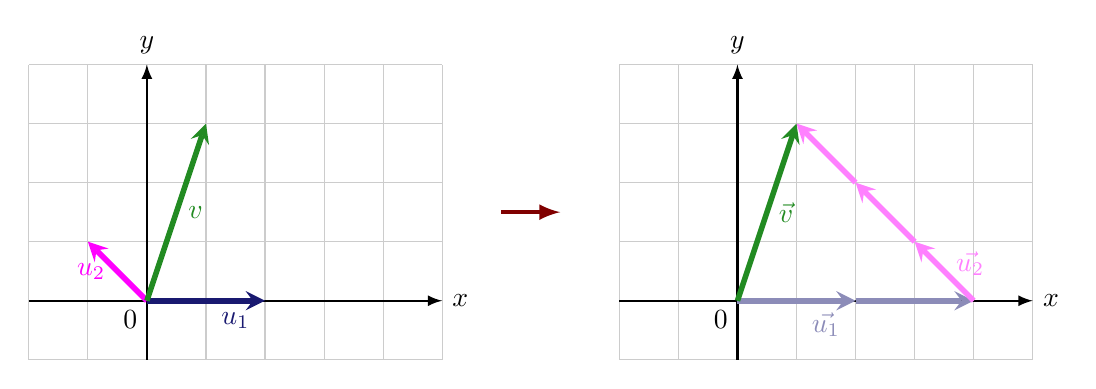
\begin{tikzpicture}[scale=0.75]
        \draw[thin,gray!40] (-2,-1) grid (5, 4);
        \draw[thick, ->, >=latex] (-2,0)--(5,0) node[right]{\(x\)};
        \draw[thick, ->, >=latex] (0,-1)--(0,4) node[above]{\(y\)};
        \draw (0, 0) node[below left] {0};
        
        \draw[line width=2pt, MidnightBlue, -stealth] (0,0)--(2,0) node[pos=3/4, below]{\(u_1\)};
        \draw[line width=2pt, Fuchsia, -stealth] (0,0)--(-1, 1) node[pos=1/2, left]{\(u_2\)};

        \draw[line width=2pt, ForestGreen, -stealth] (0,0)--(1,3) node[pos=1/2, anchor=west]{\(v\)};

        \draw[ultra thick, Maroon, ->, >=latex] (6, 1.5)--(7, 1.5);
        
        \begin{scope}[shift={(10, 0)}]
            \draw[thin,gray!40] (-2,-1) grid (5, 4);
            \draw[thick, ->, >=latex] (-2,0)--(5,0) node[right]{\(x\)};
            \draw[thick, ->, >=latex] (0,-1)--(0,4) node[above]{\(y\)};
            \draw (0, 0) node[below left] {0};
            
            \draw[line width=2pt, MidnightBlue!50, -stealth] (0,0)--(2,0) node[pos=3/4, below]{\(\vec{u_1}\)};
            \draw[line width=2pt, MidnightBlue!50, -stealth] (2,0)--(4,0);

            \draw[line width=2pt, Fuchsia!50, -stealth] (4,0)--(3, 1) node[pos=1/2, right, shift={(0, 0.1)}]{\(\vec{u_2}\)};
            \draw[line width=2pt, Fuchsia!50, -stealth] (3,1)--(2, 2);
            \draw[line width=2pt, Fuchsia!50, -stealth] (2,2)--(1, 3);

            \draw[line width=2pt, ForestGreen, -stealth] (0,0)--(1,3) node[pos=1/2, anchor=west]{\(\vec{v}\)};
        \end{scope}
        
    \end{tikzpicture}
    
    \caption{The green vector \(v\) can be expressed as a linear combination of the vectors \(u_1\) and \(u_2\), i.e. \(v = 2u_1 + 3u_2\).}
    \label{fig:Ch03-linear-comb}
\end{figure}

Given a family of vectors \(S = (\vec{u_1}, \vec{u_2}, \cdots, \vec{u_n})\), the \textit{span} of \(S\) is defined as the set of all linear combinations of the vectors in \(S\). For instance, consider the vectors shown in figure \ref{fig:Ch03-span-example}.
%
\begin{itemize}
    \item The vectors \(\vec{u}\) and \(\vec{v}\) span the \(xy\)-plane.
    \item The vectors \(\vec{u}\), \(\vec{v}\) and \(\vec{w}\) together span the entire three-dimensional space \(\mathbb{R}^3\).
    \item Since the vectors \(\vec{w}\) and \(2\vec{w}\) are collinear, their span is along a single straight line.
\end{itemize}


\tdplotsetmaincoords{60}{120}
\begin{figure}[H]
    \centering

    \begin{tikzpicture}[scale=0.75, tdplot_main_coords]
        \foreach \x in {0,1,...,5} {
            \foreach \y in {0,1,...,5} {
                \draw[thin, gray!40] (\x,-0.5) -- (\x,5.5);
                \draw[thin, gray!40] (-0.5,\y) -- (5.5,\y);
            }
        }

        \draw[thick, ->, >=latex] (0,0,0)--(5.5,0,0) node[left]{\(x\)};
        \draw[thick, ->, >=latex] (0,0,0)--(0,5.5,0) node[above]{\(y\)};
        \draw[thick, ->, >=latex] (0,0,0)--(0,0,5) node[right]{\(z\)};
        \draw (0, 0) node[above left] {0};
        
        \draw[line width=2pt, MidnightBlue, -stealth] (0,0)--(3,2) node[pos=3/4, left]{\(\vec{u}\)};
        \draw[line width=2pt, Fuchsia, -stealth] (0,0)--(1, 4) node[pos=3/4, below]{\(\vec{v}\)};
        
        \draw[line width=1pt, dashed, darkgray] (-4.5, -6, -6) -- (9, 12, 12);
        \draw[line width=2pt, ForestGreen, -stealth] (0,0,0)--(6, 8, 8) node[above]{\(2\vec{w}\)};
        \draw[line width=2pt, BurntOrange, -stealth] (0,0,0)--(3, 4, 4) node[pos=1/2, right]{\(\vec{w}\)};
    \end{tikzpicture}
    
    \caption{Three vectors in \(\mathbb{R}^3\). Both \(\vec{u}\) and \(\vec{v}\) lie flat on the \(xy\)-plane. The dashed line represents the span of \(\vec{w}\) and \(2\vec{w}\).}
    \label{fig:Ch03-span-example}
\end{figure}


Given some vector space \(V\), a subset \(U\) of \(V\) is called a \textit{subspace} if it is stable under linearity (i.e. also a vector space). For example, the \(xy\)-plane is a subspace of the three-dimensional vector space \(\mathbb{R}^3\).


\subsection{Linear independence}

The idea of \textit{linear independence} can be defined in several ways.
%
\begin{quote}
    \textbf{Definition of linear independence.}

    The vectors \(\vec{u_1},\; \vec{u_2},\; \cdots,\; \vec{u_n}\) are said to be \textit{linearly independent} if:
    %
    \begin{itemize}
        \item There exist no scalars \(a_1,\; a_2,\; \cdots,\; a_n\) (not all equal to zero) such that
        %
        \begin{equation*}\label{eq:Ch03-linear-independence}
            a_1 \vec{u_1} + a_2 \vec{u_2} + \cdots + a_n \vec{u_n} = 0 \text{.} \tag{*}
        \end{equation*}

        \item None of the vectors can be expressed as a linear combination of the others.
        
        \item None of the vectors belong to the span of the others.
    \end{itemize}
    %
    These three statements are equivalent. 
    
    To prove linear independence, we can make use of the first statement and show that for equation \eqref{eq:Ch03-linear-independence} to hold, the scalars \(a_1,\; a_2,\; \cdots,\; a_n\) must all be equal to zero.

    To disprove linear independence, we can use the second statement and show that one of the vectors can be expressed as a linear combination of the others. (Alternatively, we can provide a solution to equation \eqref{eq:Ch03-linear-independence} where not all of \(a_1,\; a_2,\; \cdots,\; a_n\) are zero.)
\end{quote}

For example, in figure \ref{fig:Ch03-span-example}, the vectors \(\vec{u}\), \(\vec{v}\) and \(\vec{w}\) are linearly independent as none of the vectors belong to the span of the others.

The example problems below demonstrate how linear independence can be proved or disproved.

\vspace{15pt}
\begin{mdframed}[linewidth=1pt]
\noindent \textbf{Problem.} Is this family of polynomials linearly independent? Explain.
%
\[\{3x,\; 4x^2 - 6x,\; 2x^2\}\] 

\textbf{Solution 1.} No. This is because one of the polynomials can be written as a linear combination of the others:
%
\[4x^2 - 6x = 2{\color{BrickRed}(2x^2)} + (-2){\color{MidnightBlue}(3x)}\]

\textbf{Solution 2.} No, because \(2{\color{MidnightBlue}(3x)} + {\color{ForestGreen}(4x^2 - 6x)} - 2{\color{BrickRed}(2x^2)}= 0\).
\vspace{10pt}
\end{mdframed}


\vspace{15pt}
\begin{mdframed}[linewidth=1pt]
\noindent \textbf{Problem.} Is this family of vectors linearly independent? Explain.
%
\[
\left\{
\begin{bmatrix}
    2 \\ 2
\end{bmatrix}
,\;
\begin{bmatrix}
    1 \\ -1
\end{bmatrix}
\right\}
\]

\textbf{Solution.} Yes. Assume there exists a linear combination such that
%
\[
a_1
\begin{bmatrix}
    2 \\ 2
\end{bmatrix}
+
a_2
\begin{bmatrix}
    1 \\ -1
\end{bmatrix}
= 0\text{.}
\]
%
This produces the following system of simultaneous equations:
%
\[
\begin{cases}
    2a_1 + a_2 = 0\\
    2a_1 - a_2 = 0
\end{cases}
\]
%
for which the only solution is \(a_1 = a_2 = 0\). Hence, the family of vectors are indeed linearly independent.
\vspace{10pt}
\end{mdframed}




\subsection{Basis}

Let \(V\) be a vector space. A basis\footnote{Plural: bases.} of \(V\) is a set \(S\) of linearly independent vectors that spans the entirety of \(V\). For instance, in figure \ref{fig:Ch03-span-example}, the set of vectors \(\{\vec{u}, \vec{v}\}\) is a basis of the \(xy\)-plane.

If the basis \(S\) is finite, then the size (cardinality) of \(S\) is referred to as the \textit{dimension} of \(V\). This means that the \(xy\)-plane in figure \ref{fig:Ch03-span-example} has a dimension of \(2\).

One of the most obvious bases for \(\mathbb{R}^n\) is
%
\[
\left\{
\begin{bmatrix}
    1 \\ 0 \\ 0 \\ \vdots \\ 0
\end{bmatrix},\;
%
\begin{bmatrix}
    0 \\ 1 \\ 0 \\ \vdots \\ 0
\end{bmatrix},\;
%
\begin{bmatrix}
    0 \\ 0 \\ 1 \\ \vdots \\ 0
\end{bmatrix},\;
%
\cdots,\;
%
\begin{bmatrix}
    0 \\ 0 \\ 0 \\ \vdots \\ 1
\end{bmatrix}
\right\}
\]
%
which is known as the \textit{canonical basis}. See figures \ref{fig:Ch03-canonical-basis-2d} and \ref{fig:Ch03-canonical-basis-3d}.

\begin{figure}[H]
    \centering

    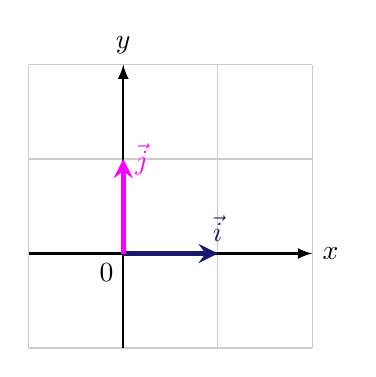
\begin{tikzpicture}[scale=1.2]
        \draw[thin,gray!40] (-1,-1) grid (2, 2);
        \draw[thick, ->, >=latex] (-1,0)--(2,0) node[right]{\(x\)};
        \draw[thick, ->, >=latex] (0,-1)--(0,2) node[above]{\(y\)};
        \draw (0, 0) node[below left] {0};
        
        \draw[line width=2pt, MidnightBlue, -stealth] (0,0)--(1,0) node[above]{\(\vec{i}\)};  
        \draw[line width=2pt, Fuchsia, -stealth] (0,0)--(0,1) node[right]{\(\vec{j}\)};
    \end{tikzpicture}
    
    \caption{The canonical basis \(\{\vec{i}, \vec{j}\}\) of \(\mathbb{R}^2\).}
    \label{fig:Ch03-canonical-basis-2d}
\end{figure}



\tdplotsetmaincoords{60}{120}
\begin{figure}[H]
    \centering

    \begin{tikzpicture}[scale=1.2, tdplot_main_coords]
        \foreach \x in {0,1,2} {
            \foreach \y in {0,1,2} {
                \draw[thin, gray!40] (\x,-0.5) -- (\x,2.5);
                \draw[thin, gray!40] (-0.5,\y) -- (2.5,\y);
            }
        }

        \draw[thick, ->, >=latex] (0,0,0)--(2.5,0,0) node[left]{\(x\)};
        \draw[thick, ->, >=latex] (0,0,0)--(0,2.5,0) node[above]{\(y\)};
        \draw[thick, ->, >=latex] (0,0,0)--(0,0,2.5) node[right]{\(z\)};
        \draw (0, 0) node[above left] {0};
        
        \draw[line width=2pt, MidnightBlue, -stealth] (0,0)--(1,0) node[pos=3/4, above left]{\(\vec{i}\)};
        \draw[line width=2pt, Fuchsia, -stealth] (0,0)--(0, 1) node[pos=3/4, above]{\(\vec{j}\)};
        \draw[line width=2pt, BurntOrange, -stealth] (0,0,0)--(0, 0, 1) node[above right]{\(\vec{k}\)};
    \end{tikzpicture}
    
    \caption{The canonical basis \(\{\vec{i}, \vec{j}, \vec{k}\}\) of \(\mathbb{R}^3\).}
    \label{fig:Ch03-canonical-basis-3d}
\end{figure}





\subsection{Linear maps}

We define a \textit{linear map} or \textit{linear mapping} as follows.
%
\begin{quote}
    \textbf{Definition of a linear map.}

    For two \(K\)-vector spaces \(V\) and \(W\), consider a function \(f : V \to W\) that maps each vector in \(V\) to a vector in \(W\).
    
    This function is said to be a \textit{linear map} if, for any two vectors \(\vec{u}, \vec{v} \in V\) and any scalar \(a \in K\), we have
    %
    \begin{align*}
        f(\vec{u} + \vec{v}) &= f(\vec{u}) + f(\vec{v})\\
        f(a\vec{u}) &= a f(\vec{u})\text{.}
    \end{align*}
\end{quote}

Once again we can combine the two equations above to get an alternative but equivalent definition.
%
\begin{quote}
    \textbf{Alternative definition of a linear map.}
    
    The function \(f : V \to W\) is said to be a \textit{linear map} if, for any two vectors \(\vec{u}, \vec{v} \in V\) and any scalar \(a \in K\), we have \(f(a\vec{u} + \vec{v}) = a f(\vec{u}) + f(\vec{v})\).
\end{quote}
%
For any linear map \(f\) we must have \(f(\vec{0}) = \vec{0}\). This can be shown by setting \(a = 0\) and \(\vec{v} = \vec{0}\) in the definition above.

An example of a linear map in \(\mathbb{R}^2\) is a function \(f\) that rotates vectors by \(90\degree\) anticlockwise, i.e.
%
\[
f\left(
    \begin{bmatrix}
        x \\ y
    \end{bmatrix}
\right)
=
\begin{bmatrix}
    -y \\ x
\end{bmatrix}
\]
%
To prove this, consider any two vectors \(\vec{u} = \begin{bmatrix} x_1 \\ y_1 \end{bmatrix}\) and \(\vec{v} = \begin{bmatrix} x_2 \\ y_2 \end{bmatrix}\). For any scalar \(a \in \mathbb{R}\), we have
%
\begin{align*}
    f(a\vec{u} + \vec{v}) &= f\left(a \begin{bmatrix} x_1 \\ y_1 \end{bmatrix} + \begin{bmatrix} x_2 \\ y_2 \end{bmatrix}\right)\\
    &= f\left(\begin{bmatrix} ax_1 \\ ay_1 \end{bmatrix} + \begin{bmatrix} x_2 \\ y_2 \end{bmatrix}\right)\\
    &= f\left(\begin{bmatrix} ax_1 + x_2 \\ ay_1 + y_2\end{bmatrix}\right)\\
    &= \begin{bmatrix} - ay_1 - y_2\\ ax_1 + x_2\end{bmatrix}\\
    &= \begin{bmatrix} - ay_1\\ ax_1\end{bmatrix} + \begin{bmatrix} - y_2\\ x_2\end{bmatrix}\\
    &= a \begin{bmatrix} - y_1\\ x_1\end{bmatrix} + \begin{bmatrix} - y_2\\ x_2\end{bmatrix}\\
    &= a f\left(\begin{bmatrix} x_1 \\ y_1 \end{bmatrix}\right) + f\left(\begin{bmatrix} x_2 \\ y _ 2 \end{bmatrix}\right)\\
    &= a f(\vec{u}) + f(\vec{v})
\end{align*}
%
which shows that \(f\) is a linear map. In fact, rotations, scalings and projections are all examples of linear maps in \(\mathbb{R}^2\).

If a linear map maps vectors from a vector space to the same vector space, i.e.
%
\[f: V \to V\]
%
then this mapping is known as an \textit{endomorphism}\footnote{From ``endo-'' (meaning ``internal'' in Greek) and ``morphism'' (a mathematical term for structure-preserving mappings).}. For instance, the \(90\degree\) rotation function we saw before maps vectors in \(\mathbb{R}^2\) to vectors in \(\mathbb{R}^2\), so it is an endomorphism.

Let \(U\), \(V\) and \(W\) be vector spaces. Given two linear maps:
%
\begin{align*}
    f: U &\to V\\
    g: V &\to W
\end{align*}
%
we can \textit{compose} them into a new linear map
%
\[g \circ f : U \to W\]
%
where \(f\) is applied first, then \(g\).





\subsection{Kernel and image}

Consider the linear map \(f : V \to W\), where \(V\) and \(W\) are vector spaces. We define the following:
%
\begin{itemize}
    \item The \textit{kernel} of \(f\), denoted as \(\kernel(f)\), is the set of vectors \(v \in V\) for which \(f(v) = \vec{0}\).
    \item The \textit{image} of \(f\), denoted as \(\image(f)\), is the set of \(f(v)\) for every \(v \in V\).
\end{itemize}
%
Both \(\kernel(f)\) and \(image(f)\) are vector spaces. Note that \(\kernel(f)\) always contains \(\vec{0}\) since \(f(\vec{0}) = \vec{0}\).

As an example, consider the following linear map.
%
\[
g\left(
    \begin{bmatrix}
        x \\ y
    \end{bmatrix}
\right)
=
\begin{bmatrix}
    x + y\\
    x + y
\end{bmatrix}
\]

To find its kernel \(\kernel(g)\), we solve
%
\begin{align*}
    g\left(
        \begin{bmatrix}
            x \\ y
        \end{bmatrix}
    \right)
    &= \vec{0} \\
    %
    \begin{bmatrix}
        x + y\\
        x + y
    \end{bmatrix}
    &=
    \begin{bmatrix}
        0\\
        0
    \end{bmatrix}\\
    %
    x + y &= 0\\
    y &= -x
\end{align*}
%
which gives us
%
\[
\kernel(g) =
%
\left\{\left.
    \begin{bmatrix}
        x \\ -x
    \end{bmatrix}
    \right|
    x \in \mathbb{R}
\right\}
%
= \Span\left(
    \begin{bmatrix}
        1 \\ -1
    \end{bmatrix}
\right)
\text{.}
\]

To find the image \(\image(g)\), we want to look for vectors \(\vec{v}\) that verify \(g(\vec{u}) = \vec{v}\) for some \(\vec{u}\). To do this, it might be useful to look at some examples and search for patterns.
%
\begin{align*}
    g\left(
        \begin{bmatrix}
            1 \\ 2
        \end{bmatrix}
    \right)
    &= \begin{bmatrix}
        3 \\ 3
    \end{bmatrix} \\
    g\left(
        \begin{bmatrix}
            3 \\ 4
        \end{bmatrix}
    \right)
    &= \begin{bmatrix}
        7 \\ 7
    \end{bmatrix} \\
    g\left(
        \begin{bmatrix}
            -5 \\ 3
        \end{bmatrix}
    \right)
    &= \begin{bmatrix}
        -2 \\ -2
    \end{bmatrix}
\end{align*}
%
We notice that the entries in the output vectors are always identical. We formalise this as follows --- for \(\vec{v} = g(\vec{u})\) to be true, we must have
%
\begin{align*}
    \exists x, y,\; \vec{v} &= \begin{bmatrix} x + y \\ x + y \end{bmatrix}\\
    \exists z,\; \vec{v} &= \begin{bmatrix} z \\ z \end{bmatrix}
\end{align*}
%
which yields \(\image(g) = \Span\left(\begin{bmatrix} 1 \\ 1 \end{bmatrix}\right)\).

